% !TEX root =  MAIN.tex

\newpage
\subsection{Developed Toolset - SEMuS}
\label{sec:semus}

\STARTCHANGEDWPT

%\DONE{This is the sentence in which you want to explain what is the solution implemented in FAQAS. You have to wrte something like "To achieve test suite augmentation (i.e., automatically generate test cases that kill mutants), in FAQAS, we have implemented an extension of SEMu that we call..."}

To achieve \INDEX{test suite augmentation} (i.e., automatically generate test cases that kill mutants), in FAQAS, we have implemented an extension of SEMu that we call SEMu for Space Software (\INDEX{SEMuS}).

%Symbolic Execution-based Mutant analysis for Space software (FAQAS-SEMuS), is an extension of SEMu that implements test generation for space software. 

% \TODO{I've extended the following paragraph; please check}

In the FAQAS context, we cannot use SEMu as it is, since it requires mutants to be compiled with the \INDEX{LLVM compiler} in LLVM-IR format. As explained previously (1) our case studies relies on compiler pipelines (e.g., RTEMS) that include architecture-specific optimizations that are not supported by LLVM, (2) there is no guarantee that the compiled objects produced by LLVM are equivalent to those produced by the original compiler, and (3) LLVM optimizations are often applied at runtime, which is infeasible when the software under test needs to be executed within a dedicated simulator (e.g., a SVF facility). The practical consequence is that the test suites of our case study systems, and, more in general, integration and system test suites of space software, cannot be used to test LLVM versions of the SUT. 
Therefore, they cannot be used to identify killed and live mutants, as a consequence, it is not possible to determine which additional test cases need to be generated. 
The solution to this problem consists of first executing \INDEX{MASS} to identify killed and live mutants, and then compile only the live mutants into LLVM-IR format. 
To minimize the limitations above, instead of compiling the whole software, we compile only the mutated function and its dependencies, which enables the generation of unit test cases, which shall be sufficient to ensure the quality of the system under test in this context (e.g., unit test cases are normally used to ensure high code coverage). To enable the compilation of such mutants, we have extended MASS to generate both a meta-mutant processed by SEMu and mutants that, after mutation analysis, can be traced back to such meta-mutant.

% !TEX root =  ../MAIN.tex



\begin{lstlisting}[style=CStyle, float=h, caption=Function T\_INT\_IsConstraintValid., label=original_meta]
flag T_INT_IsConstraintValid(const T_INT* pVal, int* pErrCode)
{
    flag ret = TRUE;
    (void)pVal;

    ret = ((*(pVal)) <= 50UL);
    *pErrCode = ret ? 0 :  ERR_T_INT;

    return ret;
}
\end{lstlisting}

\begin{lstlisting}[style=CStyle, float=h, caption=Mutant 1 of function T\_INT\_IsConstraintValid., label=meta_mutant_1]
flag T_INT_IsConstraintValid(const T_INT* pVal, int* pErrCode)
{
    flag ret = TRUE;
    (void)pVal;

    ret = ((*(pVal)) <= 50UL);
    *pErrCode = ret ? 1 :  ERR_T_INT;

    return ret;
}
\end{lstlisting}

\begin{lstlisting}[style=CStyle, float=h, caption=Mutant 2 of function T\_INT\_IsConstraintValid., label=meta_mutant_2]
flag T_INT_IsConstraintValid(const T_INT* pVal, int* pErrCode)
{
    flag ret = TRUE;
    (void)pVal;

    ret = ((*(pVal)) <= 50UL);
    *pErrCode = ret ? (-1) :  ERR_T_INT;

    return ret;
}
\end{lstlisting}

\begin{lstlisting}[style=CStyle, float=h, caption=Meta-Mutant for function T\_INT\_IsConstraintValid., label=meta_mutant_example]
flag T_INT_IsConstraintValid(const T_INT* pVal, int* pErrCode)
{
    flag ret = TRUE;
    (void)pVal;

    ret = ((*(pVal)) <= 50UL);

    klee_semu_GenMu_Mutant_ID_Selector_Func(1,2);
    *pErrCode = ret ? 
    	( klee_semu_GenMu_Mutant_ID_Selector==2 ?
    		((-1)):
		    (klee_semu_GenMu_Mutant_ID_Selector==1?
			    (1):
			    (0))) 
			    :  ERR_T_INT;
    klee_semu_GenMu_Post_Mutation_Point_Func(0,0);
    klee_semu_GenMu_Post_Mutation_Point_Func(1,2);

    return ret;
}
\end{lstlisting}

Listing~\ref{meta_mutant_example} introduces an example of a \INDEX{meta-mutant}, while Listings~\ref{meta_mutant_1} and~\ref{meta_mutant_2} introduce an example of single mutants generated by MASS for the same statement.
The meta-mutant of Listing~\ref{meta_mutant_example} shows how KLEE-SEMu introduces two mutations within the same source code; to this end, KLEE-SEMu use a set of functions for controlling the mutation at runtime within the meta-mutant, these functions are:

\begin{itemize}
	\item \texttt{klee\_semu\_GenMu\_Mutant\_ID\_Selector\_Func}: function that takes two mutant IDs as arguments, representing a range of mutant IDs.
    \item \texttt{klee\_semu\_GenMu\_Mutant\_ID\_Selector}: global variable that contains the ID of the mutant to be activated at runtime.
	\item \texttt{klee\_semu\_GenMu\_Post\_Mutation\_Poin\_Func}: This enable SEMu to do conservative pruning and remove the mutant states that are non-infected.
\end{itemize}

As shown in Listing~\ref{meta_mutant_example}, mutant 2 from Listing~\ref{meta_mutant_2} is represented on line 10, and mutant 1 from Listing~\ref{meta_mutant_1} is represented in line 12.

% \TODO{Please add an example of a meta-mutant and single mutants generated by MASS; also, add an sentence above to refer to such listings}

\begin{figure}[tb]
\begin{center}
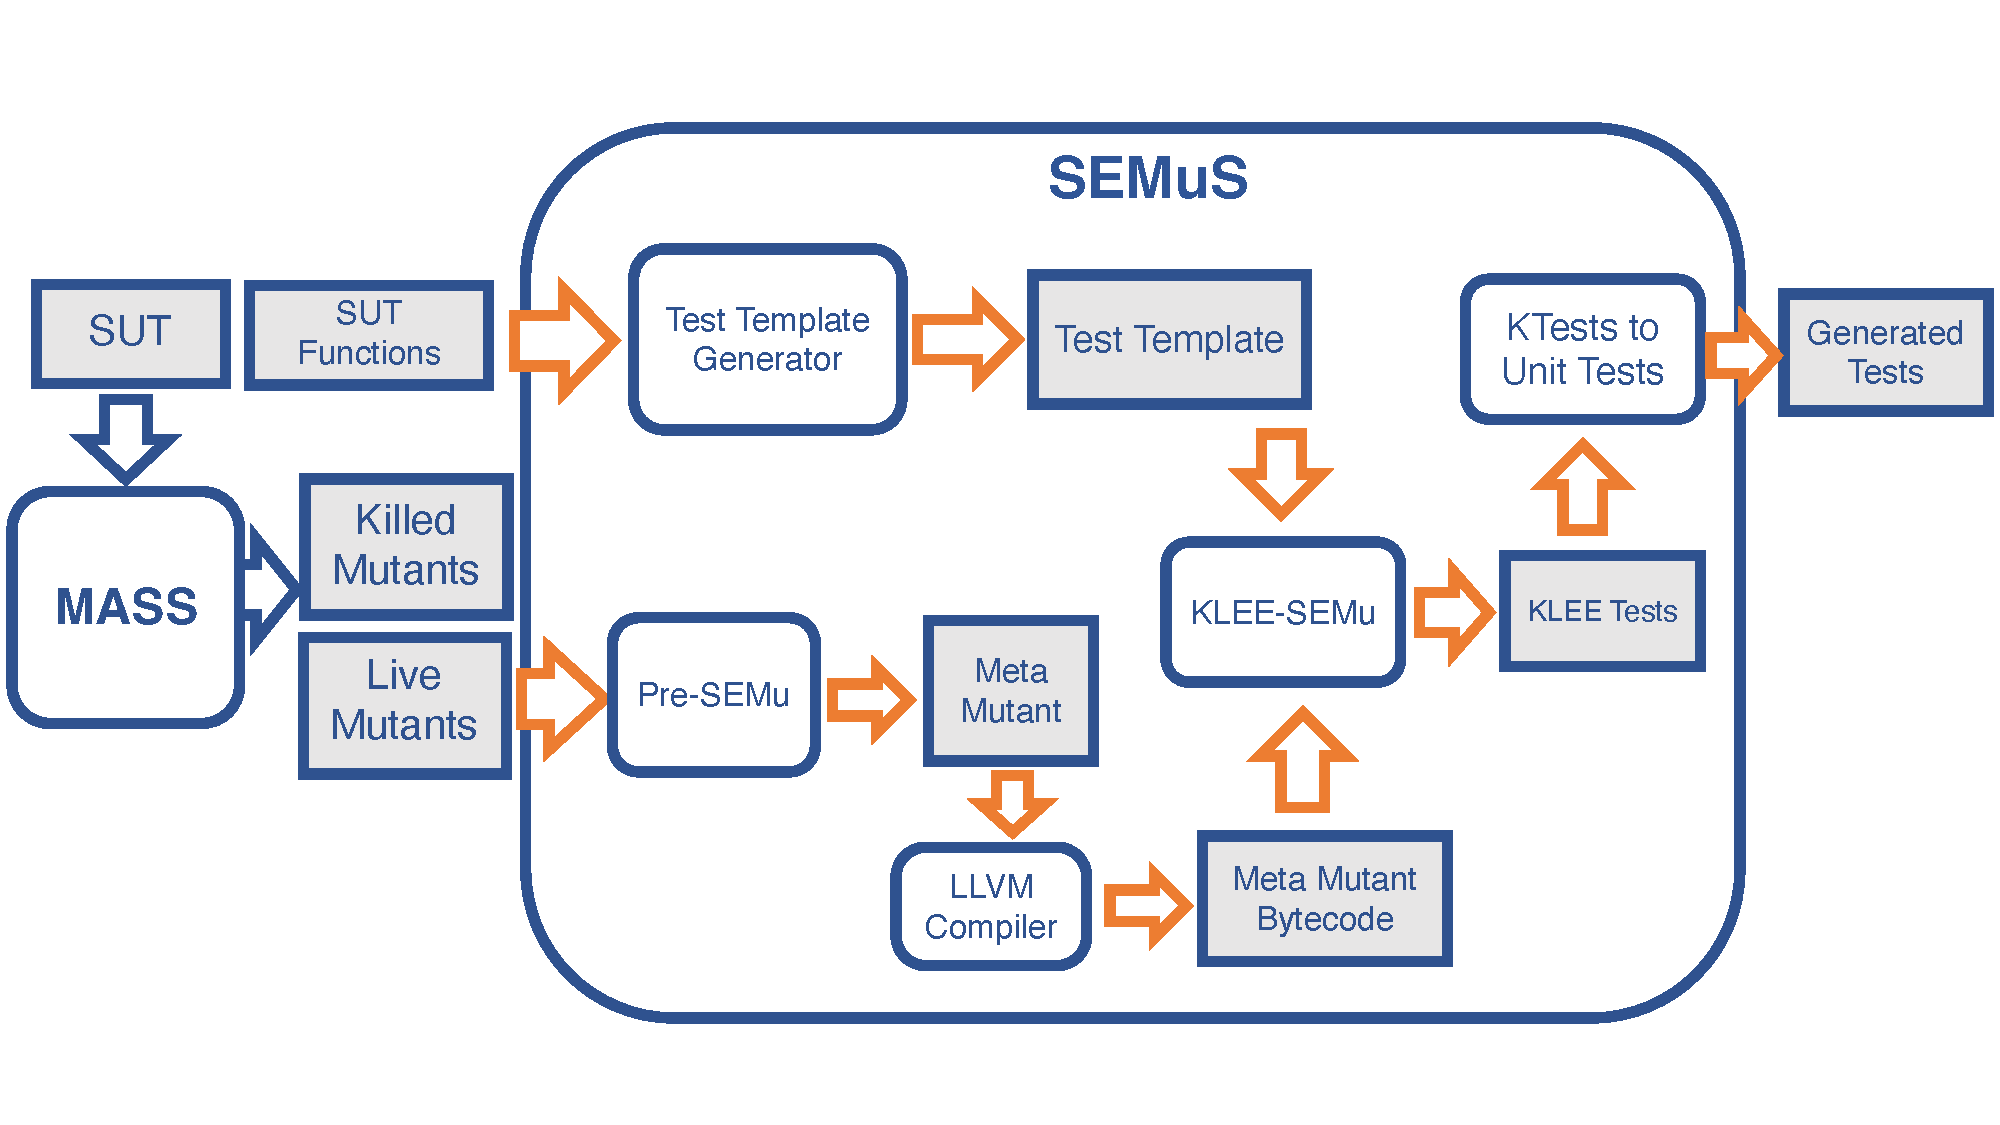
\includegraphics[width=0.8\textwidth]{images/semus-architecture}
\caption{FAQAS-SEMuS Architecture and Workflow}
\label{fig:semus_architecture}
\end{center}
\end{figure}

% !TEX root =  ../MAIN.tex

\begin{lstlisting}[style=CStyle, caption=SEMuS test template., label=test_template]
int main(int argc, char** argv) {
    // Declare variable to hold function returned value
    _Bool result_faqas_semu; 
    // Declare arguments and make input ones symbolic
    unsigned long pVal;
    int pErrCode;
    klee_make_symbolic(&pVal, sizeof(pVal), "pVal"); // Call function under test
    result_faqas_semu = T_INT_IsConstraintValid(&pVal, &pErrCode); // Make some output
    printf("FAQAS-SEMU-TEST_OUTPUT: %d\n", pErrCode);
    printf("FAQAS-SEMU-TEST_OUTPUT: %d\n", result_faqas_semu);
    return (int)result_faqas_semu;
}

\end{lstlisting}


\begin{lstlisting}[language={}, caption=Klee-test output, label=ktest]
ktest file : 'test000001.ktest'
args       : ['/MakeSym-TestGen-Input/direct/T_INT_IsConstraintValid/test.MetaMu.bc']
num objects: 2
object    0: name: b'model_version'
object    0: size: 4
object    0: data: b'\x01\x00\x00\x00'
object    1: name: b'pVal'
object    1: size: 8
object    1: data: b'\x00\x00\x00\x00\x00\x00\x00\x00'
\end{lstlisting}

Figure~\ref{fig:semus_architecture} shows the architecture of SEMuS and how it interacts with MASS. SEMuS consists of five components, which are \emph{Test Template Generator},  \emph{Pre-SEMu},  \emph{KLEE-SEMu},  \INDEX{KTest to Unit Test}, and \INDEX{LLVM}.
They enable the adoption of SEMu in the space context. In particular, SEMuS (1) automates the generation of a test template including symbolic variables that guides the generation of test inputs, and (2) compiles the test template and the mutant into the format required by SEMu (i.e., LLVM-IR). 


The \INDEX{Test Template Generator} (TTG) component automates the generation of templates for the symbolic execution search. The component receives as inputs the SUT source code and the list of SUT functions. 
Listing~\ref{test_template} shows an example of a test template generated by the TTG. The TTG generates a template for every SUT function; as shown in Listing~\ref{test_template} the component parses the function arguments and declares them symbolic through use of the KLEE function \texttt{klee\_make\_symbolic}. Then, it adds a call to the function under analysis with symbolic values, and it saves the output into the variable \texttt{result\_faqas\_semu}. Finally, the TTG adds a return call with the \texttt{result\_faqas\_semu} variable value.

The \INDEX{Pre-SEMu} component generates \INDEX{mutant schemata}; specifically, the component includes and compiles all the live mutants (i.e., MASS output) into a single bytecode file named the \emph{Meta Mutant}. At runtime, SEMu will select which mutant to consider for test generation based on a parameter. The compilation of the Meta Mutant into LLVM bitcode is supported by the \emph{LLVM} compiler infrastructure. 


% !TEX root =  ../MAIN.tex
\begin{lstlisting}[float=t, language={}, caption=Klee-test output, label=ktest]
ktest file : 'test000001.ktest'
args       : ['/MakeSym-TestGen-Input/direct/T_INT_IsConstraintValid/test.MetaMu.bc']
num objects: 2
object    0: name: b'model_version'
object    0: size: 4
object    0: data: b'\x01\x00\x00\x00'
object    1: name: b'pVal'
object    1: size: 8
object    1: data: b'\x00\x00\x00\x00\x00\x00\x00\x00'
\end{lstlisting}

\INDEX{KLEE-SEMu} is the underlying test generation component, previously described in Section~\ref{klee-semu}. This component receives as inputs the \emph{LLVM bitcode Meta Mutant} and the \emph{Test Template} for the function under test, and proceeds to apply dynamic symbolic execution to generate test inputs to kill the mutants. The output of this component are the \emph{KLEE tests}.

% \TODO{you need to list what are "the parameters of the execution"}
A \INDEX{KLEE test} is a binary file that contains information about the execution of KLEE such as the entry point of the analysis, and the generated test inputs.


An example of a KLEE test is presented in Listing~\ref{ktest}. The field \emph{args} report the entry point of the analysis; in this case, the test generation was performed for live mutants present in the function \texttt{T\_INT\_IsConstraintValid}, which SEMuS stores in a dedicated folder. The fields named \emph{object} provide information about the outputs generated by KLEE (e.g., the generated test inputs). 
For each object, the KLEE test provides a \emph{name} (usually the name of the symbolic variable), its \emph{size}, and the actual \emph{value} generated by KLEE through constraint solving (usually this is reported in binary form).
Objects are numbered. Object number \emph{0} reports information about the data structure used by KLEE, that is, the version of the structure. The other objects report information about the generated test inputs.
Our example shows that one value of size 8 was generated for the variable \texttt{pVal}, the data field shows the binary representation of the \texttt{pVal} variable, in this case \texttt{pVal=0}.


% !TEX root =  ../MAIN.tex

\begin{lstlisting}[float=t, style=CStyle,  caption=Generated test case, label=gen_test_case]
#include <stdio.h>
#include <string.h>

#include "asn1crt.c"
#include "asn1crt_encoding.c"
#include "asn1crt_encoding_uper.c"


int main(int argc, char** argv)
{
    (void)argc;
    (void)argv;

    // Declare variable to hold function returned value
    _Bool result_faqas_semu;

    // Declare arguments and make input ones symbolic
    unsigned long pVal;
    int pErrCode;
    memset(&pVal, 0, sizeof(pVal));
    const unsigned char pVal_faqas_semu_test_data[] = {0x00, 0x00, 0x00, 0x00, 0x00, 0x00, 0x00, 0x00};
    memcpy(&pVal, pVal_faqas_semu_test_data, sizeof(pVal)); // Unsigned val is 0

    // Call function under test
    result_faqas_semu = T_INT_IsConstraintValid(&pVal, &pErrCode);

    // Make some output
    printf("FAQAS-SEMU-TEST_OUTPUT: pErrCode = %d\n", pErrCode);
    printf("FAQAS-SEMU-TEST_OUTPUT: result_faqas_semu = %d\n", result_faqas_semu);
    return (int)result_faqas_semu;
}
\end{lstlisting}



The component \INDEX{KTest to Unit Test} (KTU) converts a KLEE test into a readable, executable C test case. Similar to the TTG component, the KTU uses a template to hold the specifics variables of each function under test. 
Listing~\ref{gen_test_case} shows an example of a test case generated for a mutant present in the function \texttt{T\_INT\_IsConstraintValid}. For instance, line 20 shows that the variable \texttt{pVal} is initially filled with 0 (to clean it), then in line 21, it is filled with the value stored in the variable \texttt{pVal\_faqas\_semu\_test\_data}, which holds the binary output produced by KLEE. In line 25, the function under test is invoked with the concrete value of \texttt{pVal}. Finally, the KTU print the function return value and the value of every variable passed by reference.
At the current stage, KTU does not generate assertions. Assertions need to be implemented by engineers in place of the generated \emph{printfs} because only the engineers can know, based on specifications, what are the values to be expected at the end of the test case execution.


\ENDCHANGEDWPT
